\section{Reducing The Branching Factor Further}
Consider an empty rectangle of width $w$ and height $h$ where $w > h$.  After
adding all non-dominated macro edges, each node from the perimeter will have
between $h$ to $2h-1$ neighbours from the opposite side of the rectangle, up to
2 neighbours from the same side of the rectangle and up to 5 other neighbours
from adjacent rectangles.  Such a high branching factor is undesirable as
individual node expansion operations take longer.

In this section we study two branching factor reduction methods.  The first is
an offline technique that prunes nodes from the perimeter of each rectangle.
The second is an online pruning strategy which we apply during individual node
expansion operations.  We discuss both methods in the context of 8-connected
grid maps however they are equally applicable to 4-connected maps.

\noindent
\textbf{Perimeter Reduction:}
We observe that in many cases there are nodes on the perimeter of an empty
rectangle which have no neighbours from any adjacent rectangle.  These nodes
represent intermediate locations between entry and exit points that lead into
and out of each empty rectangle. To speed up search we propose pruning from the
perimeter of each rectangle all such nodes.  To preserve optimality, we will
connect the neighbours of each pruned node directly to each other.  The weight
of each new edge is set appropriately to the octile distance between the two
neighbours.  Figure \ref{fig-branching} (Top) shows an example.  As we will see
this optimisation can have a dramatic effect on the average performance of A* on
certain types of maps.

\begin{lemma}
Perimeter reduction preserves path optimality.
\end{lemma}
\begin{proof}
Sketch: Each time we prune a node from the perimeter we add a new edge between
all its neighbours with weight equal to the distance between each pair
of neighbours.  Thus, if a path exists between a pair of nodes before the
application of perimeter reduction it is guaranteed to exist afterward.
Further, the length of this path is unchanged.
\end{proof}

\begin{figure}[t]
	\begin{center}
	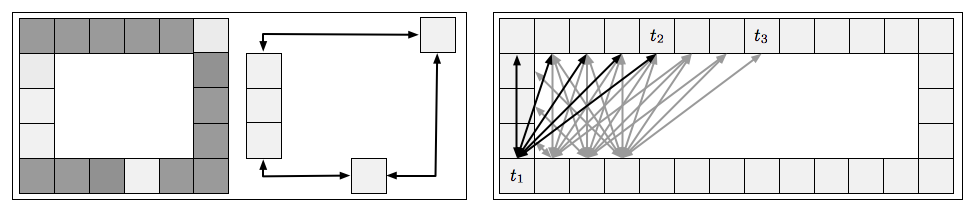
\includegraphics[width=0.97\columnwidth, trim = 10mm 10mm 10mm 0mm]
	{diagrams/branching_wide.png}
	\end{center}
	\vspace{-3pt}
	\caption{(Top) From each empty rectangle we prune all (dark grey) nodes which
	have no neighbours in any adjacent rectangle.
	Remaining nodes are then connected directly.
	(Bottom) Assume that $t_{1}$ is the parent of $t_2$. When $t_2$
	is expanded, there is no need to generate its secondary neighbors.
	These can be reached directly from $t_1$ on a shorter or equal-length path.
}
\label{fig-branching}
\end{figure}

\noindent
\textbf{Online Node Pruning:}
Given a perimeter node $n$, let us partition its macro neighbors 
(connected to $n$ by macro-edges)
on the perimeter into 
\emph{primary neighbours} and \emph{secondary neighbours}.  Secondary neighbours are those
which are located on the opposite side of the perimeter to as compared to $n$
(excluding any corner nodes).  Primary neighbours are all the rest.

When expanding an arbitrary node from the perimeter of a rectangle we observe
that it is not necessary to consider any secondary neighbours if both the node
and its predecessor belong to the same rectangle. Figure \ref{fig-branching}
(Bottom) shows an example of such a situation; any path to a secondary neighbour
is strictly dominated by an alternative path through the predecessor. 
We apply this observation as follows: {During
node expansion, determine which rectangle the parent of the current node belongs
to.} {If the current node has no parent or the parent belongs to a different
rectangle, then process (i.e., generate) all primary and secondary neighbours.
Otherwise, process only primary neighbours.}

\begin{lemma}
Online node pruning preserves path optimality.
\end{lemma}
\begin{proof}
Sketch: Let $m$ be a node on the perimeter of a rectangle. Assume that its
parent $p$ belongs to the same rectangle.  Let $n$ be a secondary successor of
$m$.  Recall that $n$ and $m$ are on opposite sides of the rectangle.  We argue
below that passing through $m$ cannot possibly improve the best path between $p$
and $n$.  Therefore, there is no need to consider $(m,n)$ macro-edges when $m$
and $p$ belong to the same rectangle.

There are 4 cases when a node $m$ and its parent $p$ belong to the same
rectangle. In case 1, $p$ is a re-inserted node from the interior of the
rectangle.  Obviously, the path segment $p,m,n$ is suboptimal, as we zigzag from
$p$ to $m$ on one side of the rectangle and then to $n$ on the opposite side of
the rectangle.  In cases 2, 3, and 4, $p$ and $m$ are on opposite sides, on
orthogonal sides or on the same side of the rectangle. As in case 1, it is
possible to check in each case that taking a detour through $m$ does not improve
the shortest path from $p$ to $n$.
\end{proof}

%Let $R$ be an empty rectangle in an 8-connected grid map.
%Further, let $m$ and $n$ be two arbitrarily selected nodes from the perimeter of $R$.
%There are three cases to consider when searching for an optimal path between $m$ and $n$:
%\begin{enumerate}
%\item{$m$ and $n$ are on the same side of the rectangle.}
%\item{$m$ and $n$ are on orthogonal sides of the rectangle.}
%\item{$m$ and $n$ are on opposite sides of the rectangle.}
%\end{enumerate}
%In all cases we begin by expanding $m$ and process all its primary and secondary neighbours.
%In the first and second case the optimal path from $m$ to $n$ involves no nodes from the opposite side of the rectangle;
%the decision to ignore all secondary neighbours has no effect on the optimality of the solution.
%In the third case we argue as follows:
%when we expand $m$ we generate a node $n'$ on the same side of the perimeter as $n$.
%The edge $(m, n')$ represents a path that crosses the rectangle from $m$ to $n'$
%using a maximum number of diagonal steps. 
%From this it is trivial to derive that the path $\lbrace m, n', n \rbrace$ is itself optimal.
%Thus we can ignore all secondary neighbours of nodes descended from $m$ in the search tree
%(evaluating them could not possibly improve the length of any path from $m$ to $n$).
%\end{proof}
%%It is worth noting that on 4-connected maps the branching factor of each node on
%%the perimeter is already constant. 
%%Applying Fast Node Expansion in this case often results in an average branching
%%factor smaller than 4. 
%%On 8-connected maps the effectiveness of this approach is dependent on how well
%%we can decomposde the grid map into large rectangular rectangles.



